\begin{frame}{Les vêtements}
  \begin{columns}
    \column{0.5\textwidth}
      Qu'est-ce qu'on met? \\
      \tinygloss{What does one put on?}
      {\small
      \begin{enumerate}
        % \item Pour aller en classe, mes amis \underline{\uncover<2->{mettent}} ...
        \item Pour manger au resto U, nous \underline{\uncover<2->{mettons}} ...
        \item Pour courir dans un marathon, tu \underline{\uncover<4->{mets}} ...
        \item Pour faire des courses, ma mère \underline{\uncover<6->{met}} ...
        \item Pour travailler dans le jardin, mon père \underline{\uncover<8->{met}} ...
        \item Pour faire du ski, je \underline{\uncover<10->{mets}} ...
        \item Pour nager, elles \underline{\uncover<12->{mettent}} ...
        \item Pour sortir avec des amis, vous \underline{\uncover<14->{mettez}} ...
      \end{enumerate}
      }
    \column{0.5\textwidth}
      \begin{minipage}[c][0.6\textheight]{\linewidth}
        \begin{center}
          % \only<1-2>{
          %   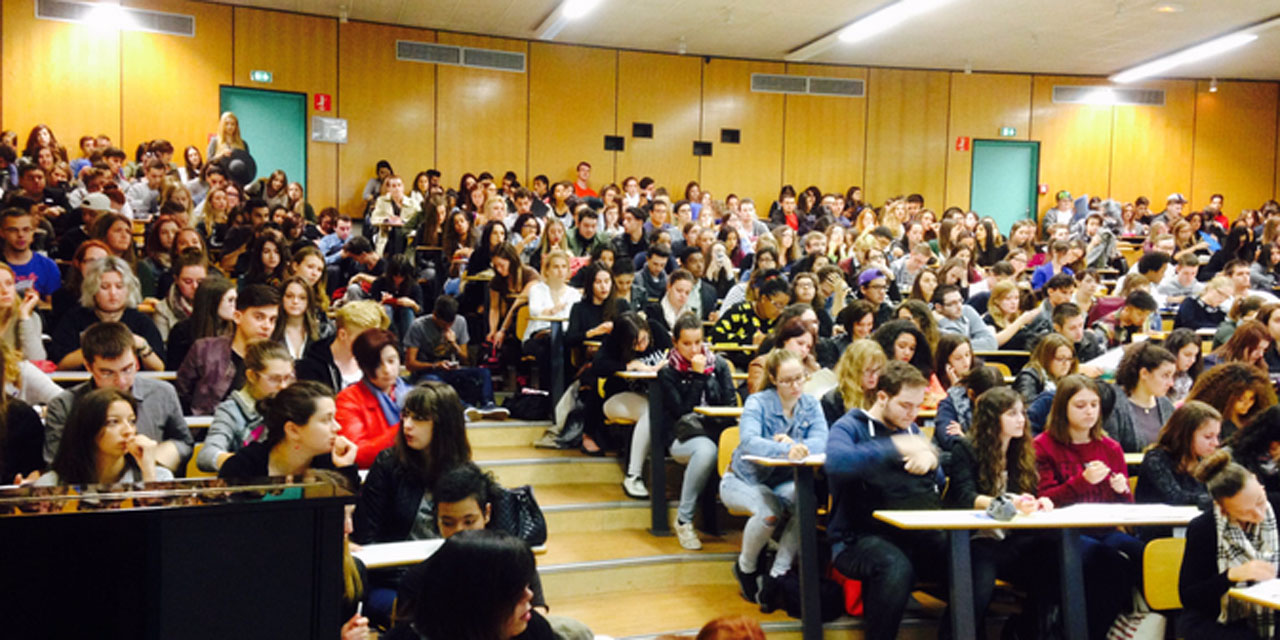
\includegraphics[scale=0.125]{classe.png}
          % }
          \only<1-2>{
            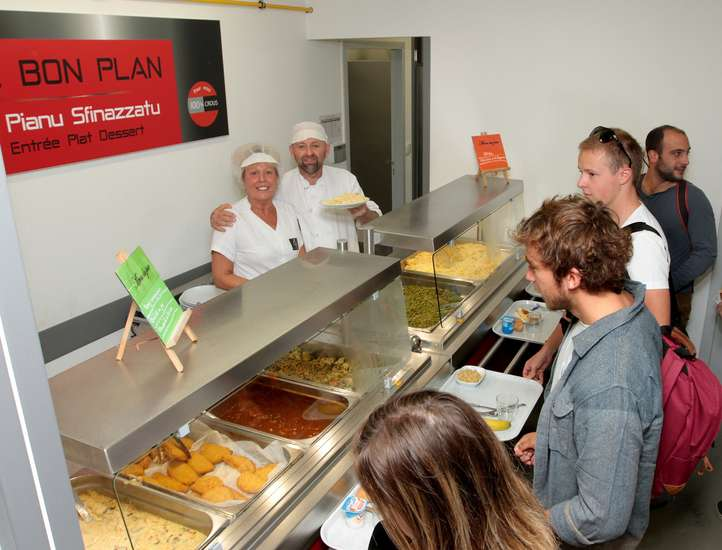
\includegraphics[scale=0.18]{restou.jpg}
          }
          \only<3-4>{
            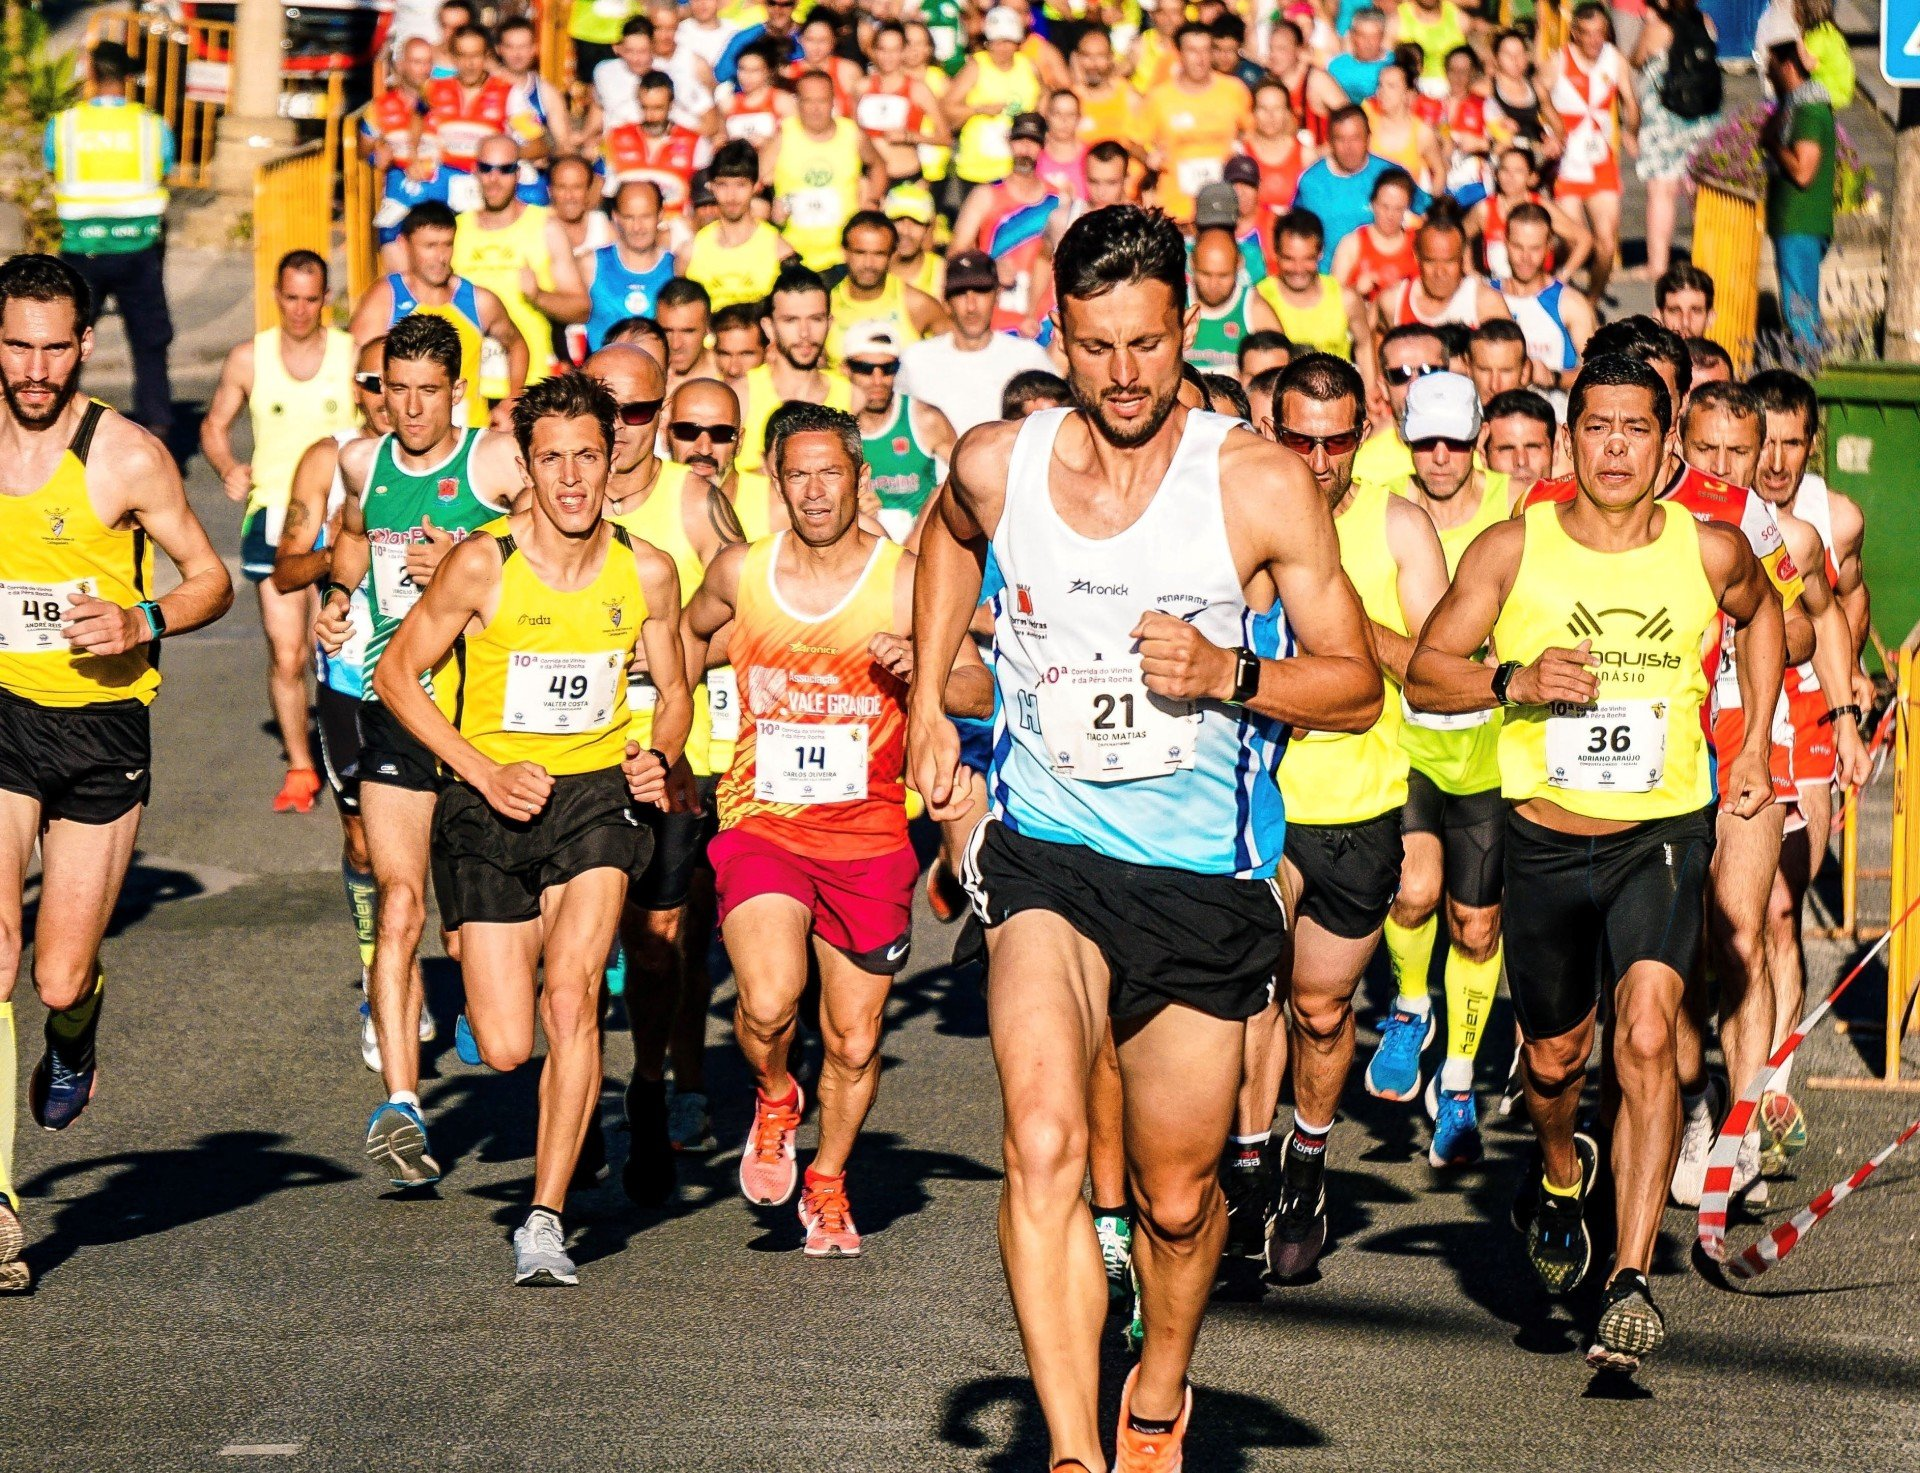
\includegraphics[scale=0.09]{marathon.jpg}
          }
          \only<5-6>{
            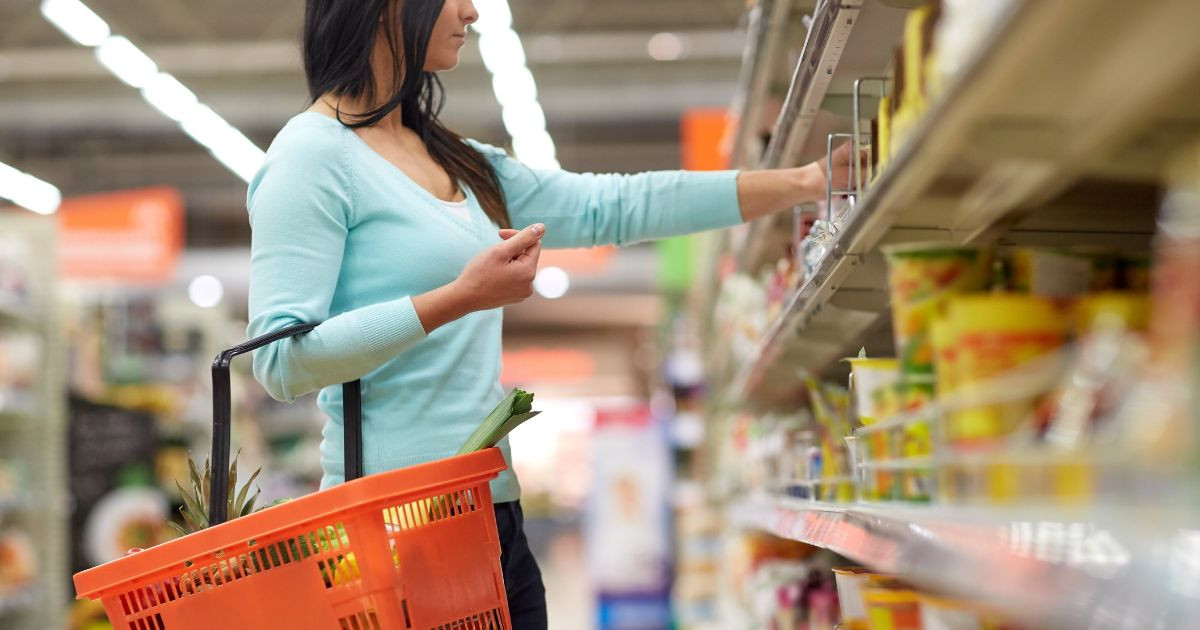
\includegraphics[scale=0.18]{courses.jpg}
          }
          \only<7-8>{
            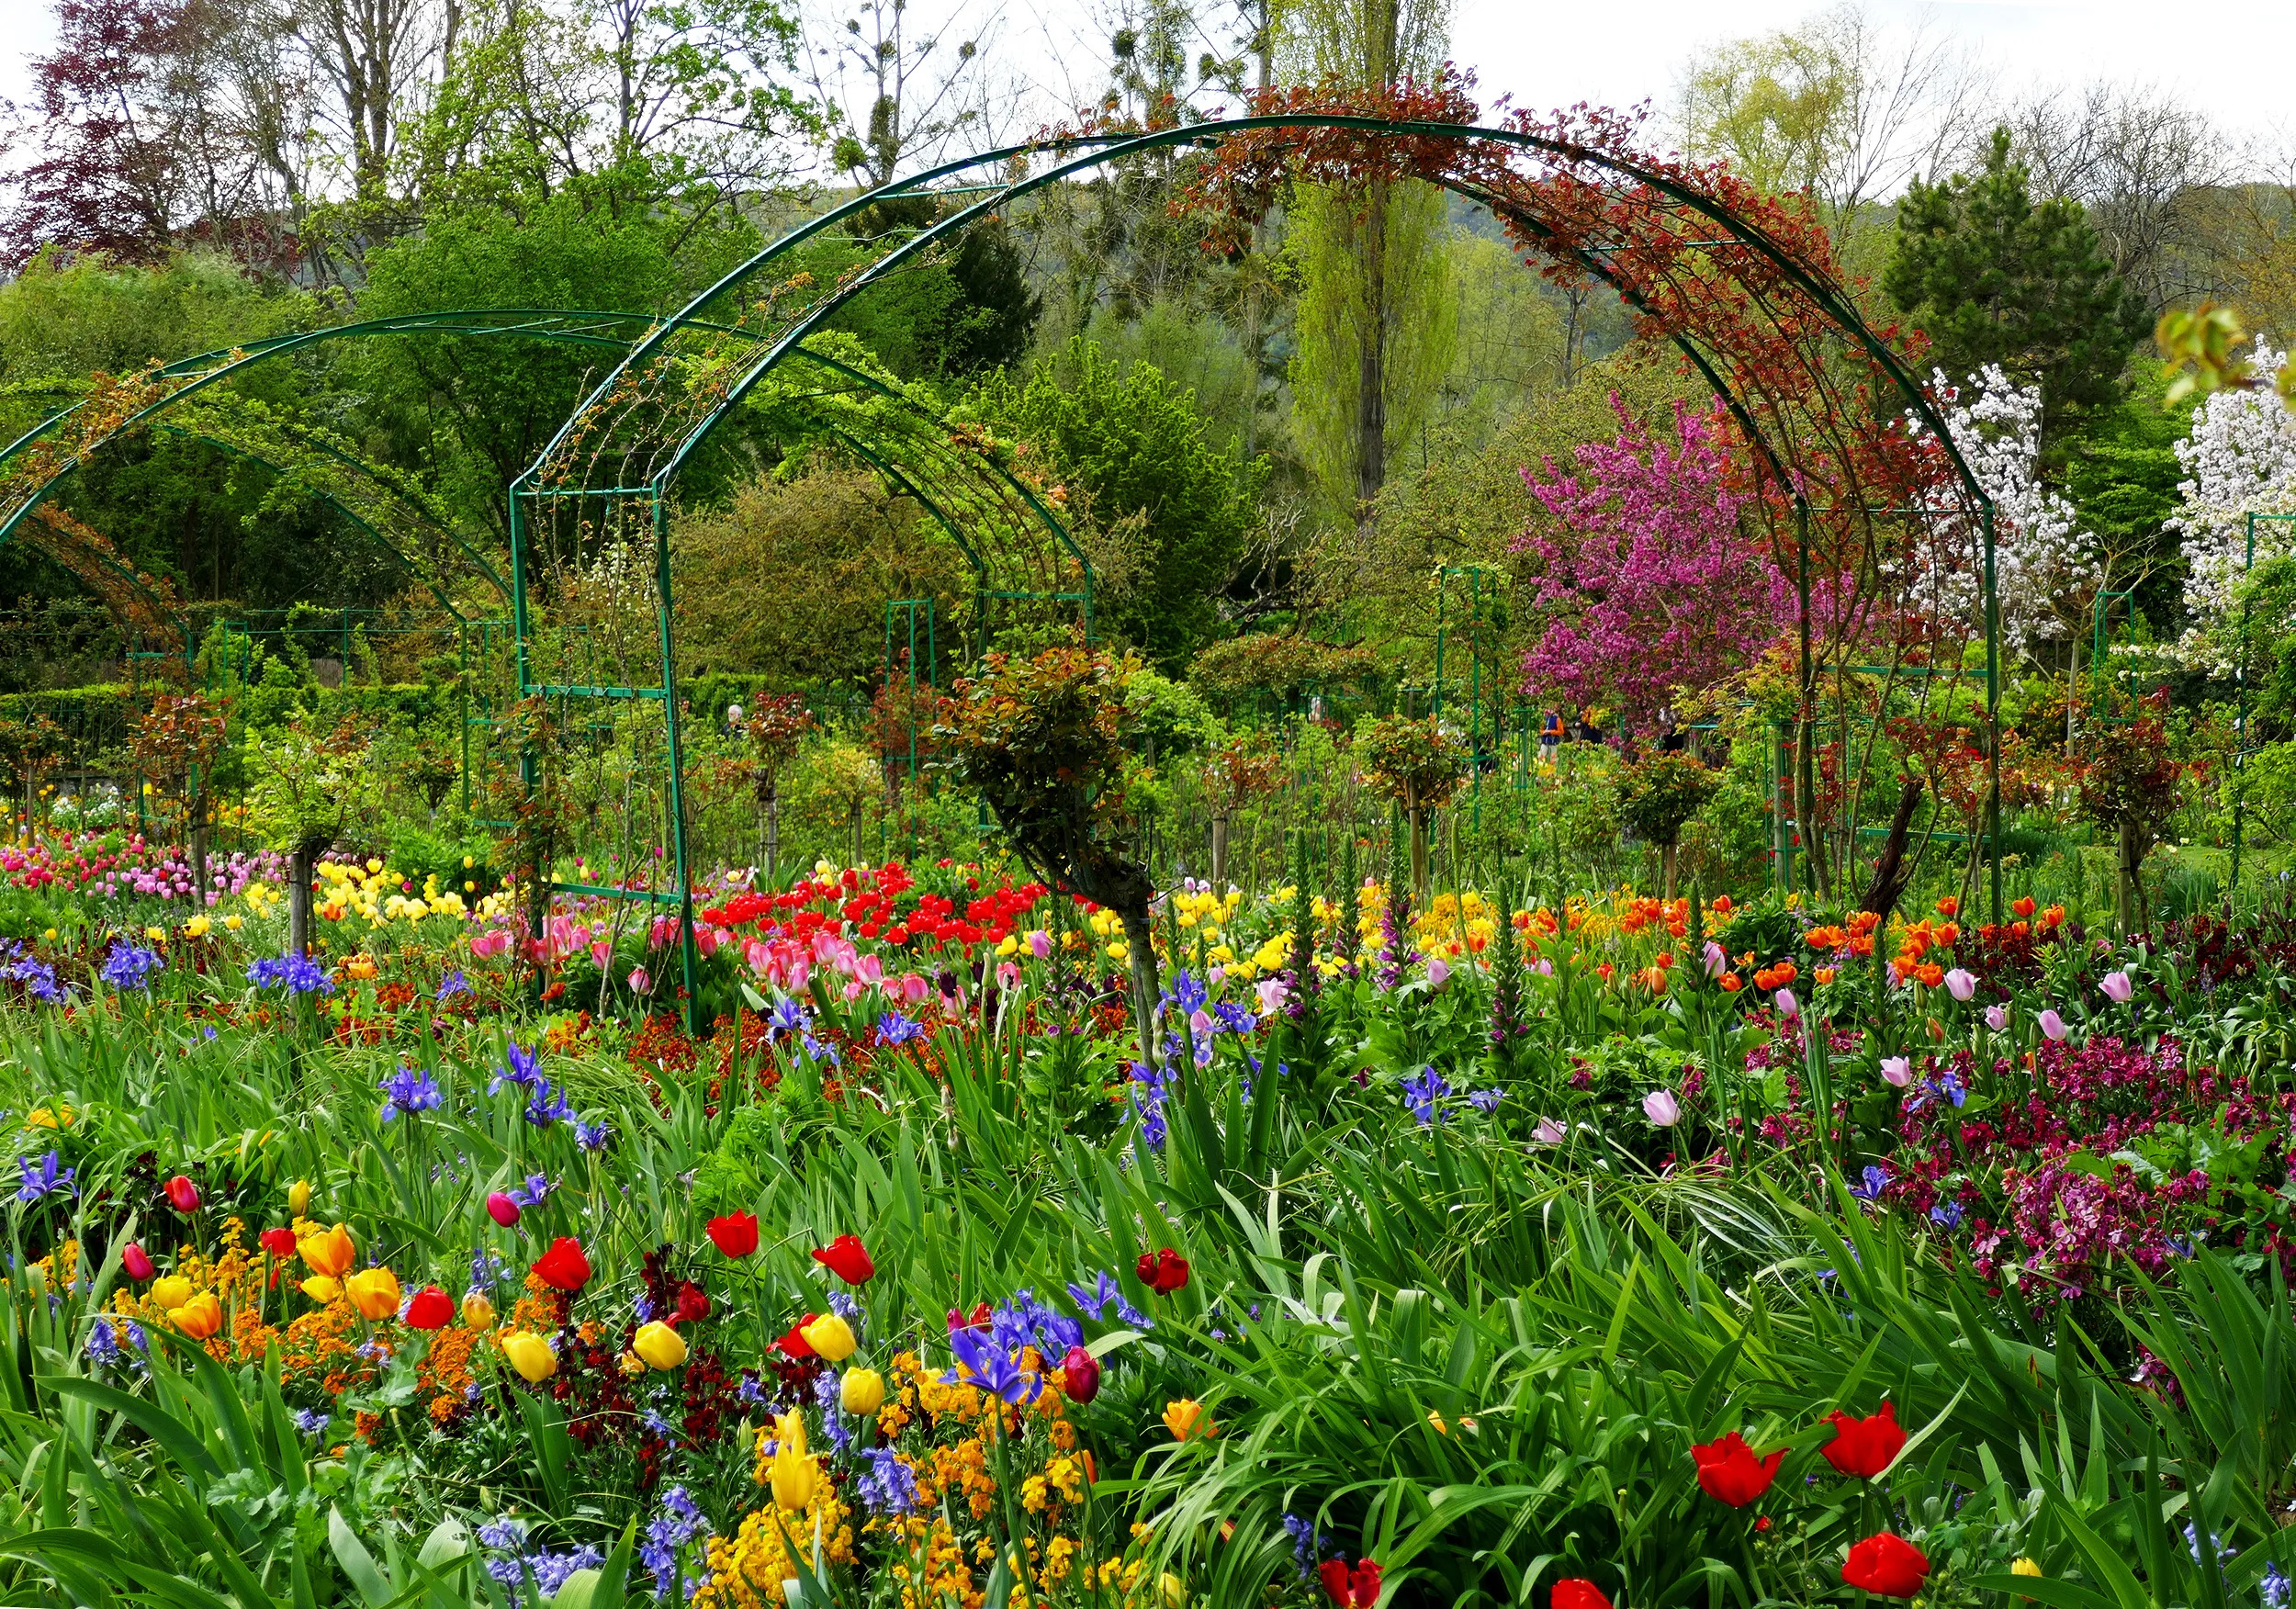
\includegraphics[scale=0.07]{giverny.jpg} \\
            Le jardin de Monet à Giverny
          }
          \only<9-10>{
            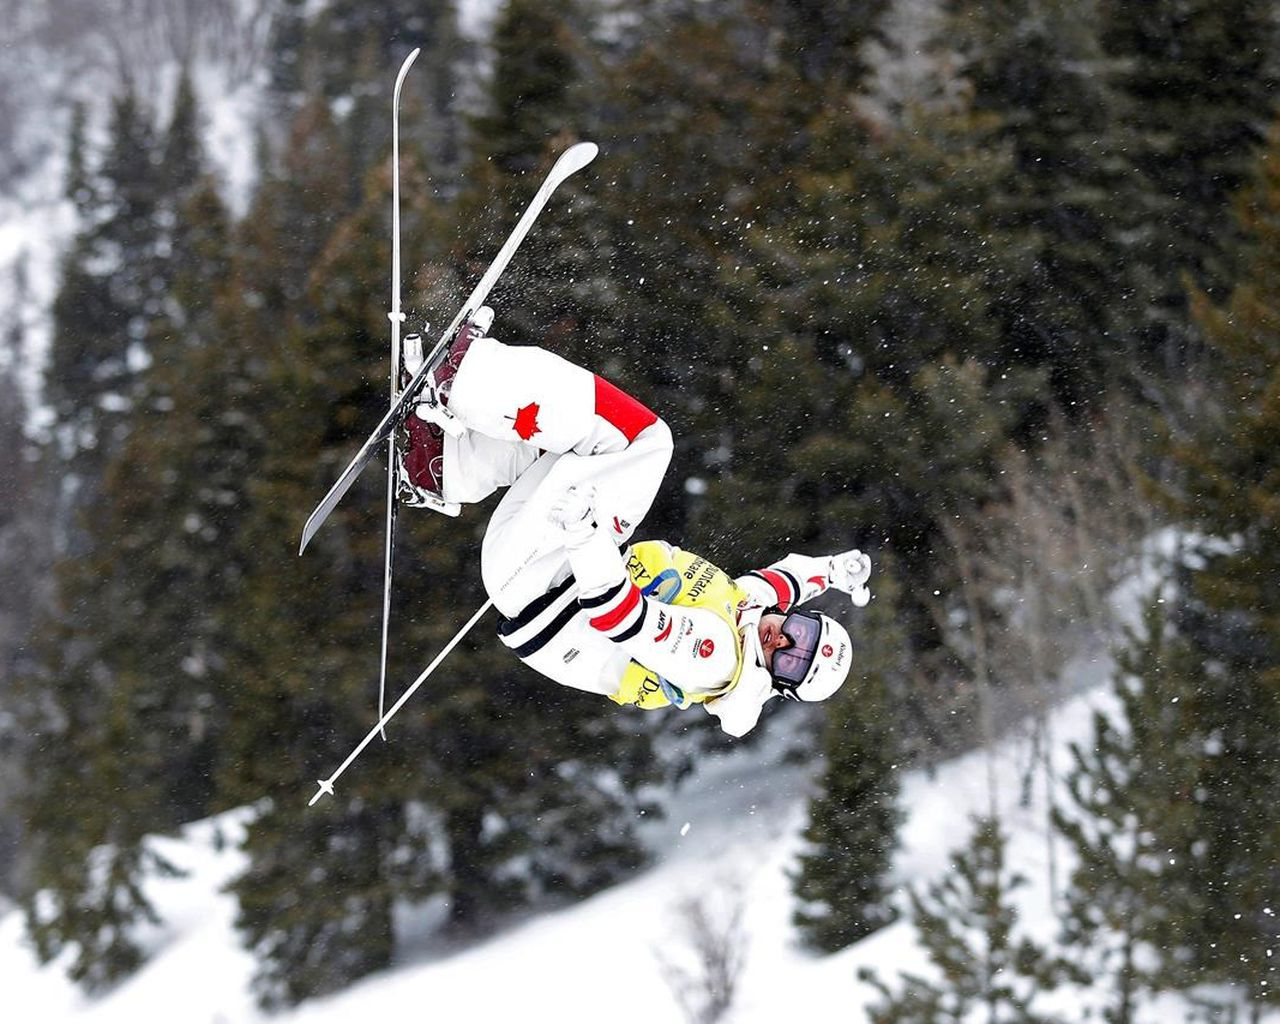
\includegraphics[scale=0.125]{kingsbury.jpg} \\
            Mikaël Kingsbury du Québec
          }
          \only<11-12>{
            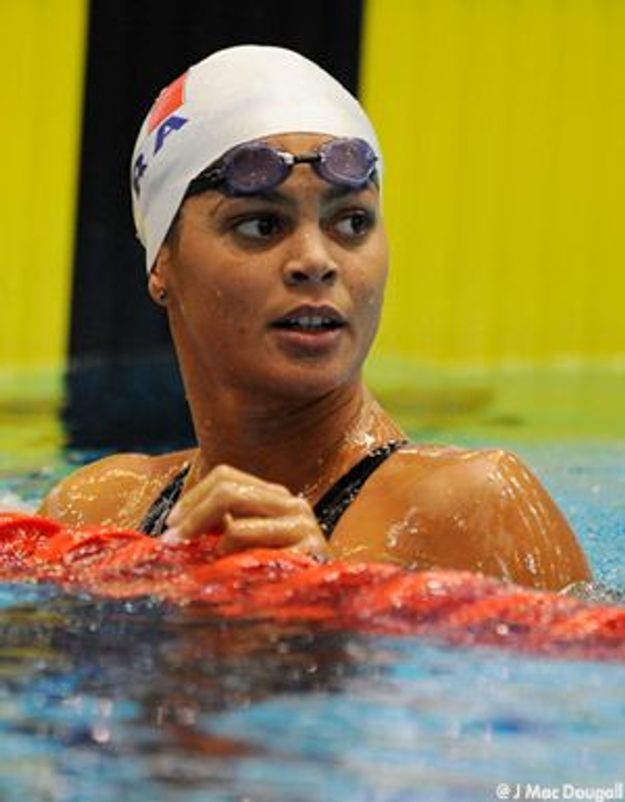
\includegraphics[scale=0.2]{balmy.jpg} \\
            Coralie Balmy de la Martinique
          }
          \only<13-14>{
            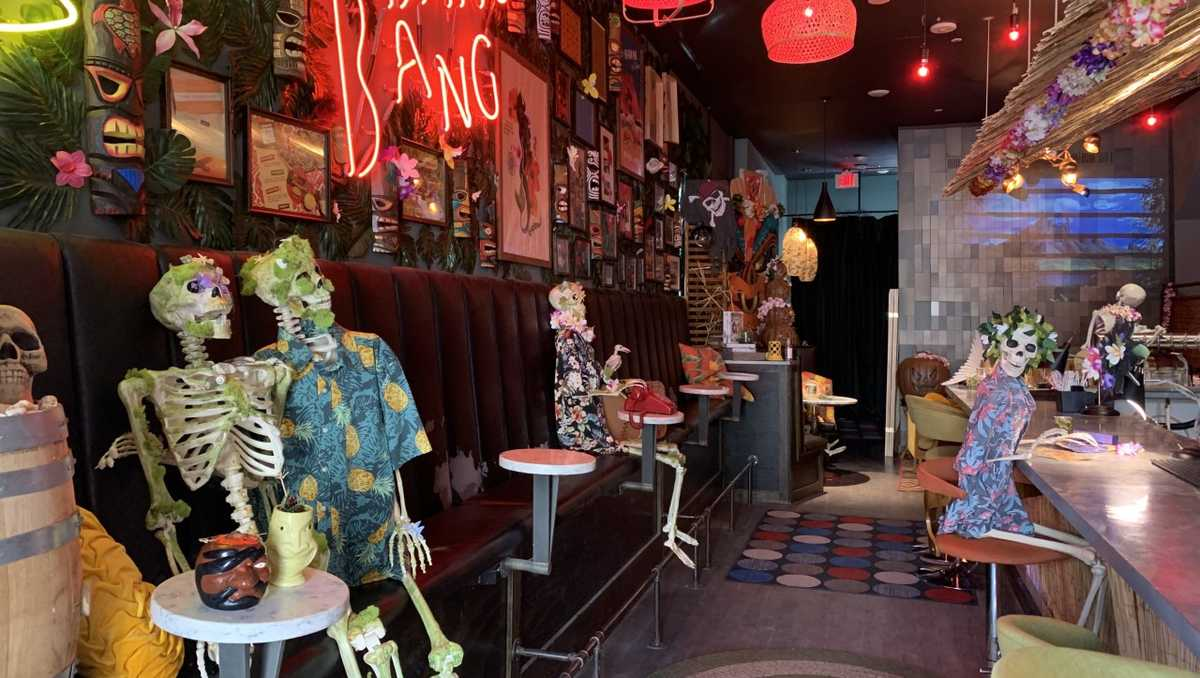
\includegraphics[scale=0.14]{bar_halloween.jpg}
          }
        \end{center}
      \end{minipage}
  \end{columns}
\end{frame}